% ============================================================================
% DDI RISK ANALYSIS WEB APPLICATION - Brief Methods and Results
% ============================================================================

\documentclass[11pt,a4paper]{article}
\usepackage[utf8]{inputenc}
\usepackage{booktabs}
\usepackage{geometry}
\usepackage{hyperref}
\usepackage{float}
\usepackage{graphicx}
\geometry{margin=1in}

\title{\textbf{DDI Risk Analysis Web Application}}
\author{Drug-Drug Interaction Knowledge Graph Project}
\date{}

\begin{document}

\maketitle

% ============================================================================
\section{Introduction}
% ============================================================================

Polypharmacy---the concurrent use of multiple medications---is increasingly common among elderly patients managing chronic conditions such as cardiovascular disease, where complex drug regimens are often necessary. However, this therapeutic complexity introduces significant risk of drug-drug interactions (DDIs) that can lead to adverse events, hospitalization, or therapeutic failure. While comprehensive DDI databases exist, their clinical utility is limited by fragmented access, lack of integration with alternative drug recommendations, and absence of natural language explanations suitable for rapid clinical decision-making. This paper presents a web-based DDI risk analysis application that addresses these barriers by integrating a large-scale biomedical knowledge graph with an intuitive three-panel interface supporting multiple input modalities (text, clinical narratives, prescription images), automated severity classification, mechanistic explanations, evidence-based alternative drug recommendations, and a locally-deployed large language model for interactive clinical consultation---enabling clinicians to rapidly assess polypharmacy risk and explore safer therapeutic options without compromising patient data privacy.

% ============================================================================
\section{System Architecture}
% ============================================================================

We developed a web-based drug-drug interaction (DDI) analysis application using the Gradio framework (Python) with a three-column responsive interface. The application is structured as follows:

\textbf{Column 1 (Input):} Accepts drug input through three tabbed modalities: (1) direct text entry supporting multiple separators (comma, plus sign, newline, ``and''), (2) clinical narrative extraction via token-level matching against the drug database, and (3) prescription image upload with optical character recognition using Tesseract-OCR/PIL. Drug names are resolved through a curated alias dictionary of 54 brand-to-generic mappings (e.g., Lipitor$\rightarrow$atorvastatin, Coumadin$\rightarrow$warfarin) and fuzzy string matching using Python's SequenceMatcher (threshold $\geq$0.95 for automatic acceptance, 0.6--0.95 suggests candidates for user confirmation). A ``Validate'' button provides interactive drug identification preview before analysis.

\textbf{Column 2 (Report):} Displays comprehensive analysis results including identified drugs, severity-classified DDI pairs (contraindicated, major, moderate, minor), risk level assessment (Critical/High/Moderate/Low), shared side effects indicating additive toxicity risk, shared protein targets explaining mechanistic overlaps, and alternative drug suggestions with risk reduction metrics. The report content is synthesized by the LLaMA 7B large language model into human-readable natural language summaries, generated as formatted Markdown with color-coded severity indicators.

\textbf{Column 3 (Assistant):} Provides an integrated LLaMA 7B chatbot served locally via Ollama (http://localhost:11434) for context-aware clinical consultation. The assistant maintains conversation history and has access to the current analysis context (drugs, interactions, alternatives) to provide informed responses about interaction mechanisms, clinical significance, and monitoring recommendations.

% ============================================================================
\section{Knowledge Graph Backend}
% ============================================================================

The application queries a multi-source biomedical knowledge graph comprising 45,655 nodes and 1,211,674 edges. Node types include: 4,313 drugs, 3,176 proteins, 5,548 side effects, 3,041 diseases, 25,958 pathways, and 3,619 drug categories.

\textbf{Edge relationships:}
\begin{itemize}
\item \textbf{Drug-Drug Interactions:} 759,774 DDIs with severity distribution: moderate (590,874; 77.8\%), minor (69,224; 9.1\%), contraindicated (44,146; 5.8\%), major (35,960; 4.7\%)
\item \textbf{Drug-Side Effect:} 265,238 associations from the SIDER database
\item \textbf{Drug-Category:} 70,618 therapeutic categorizations
\item \textbf{Drug-Disease:} 63,278 disease associations from the Comparative Toxicogenomics Database (CTD)
\item \textbf{Drug-Pathway:} 31,207 biochemical pathway mappings
\item \textbf{Drug-Protein:} 21,559 target protein relationships
\end{itemize}

\textbf{Data sources:} DrugBank (drugs, DDIs, proteins, pathways, categories), SIDER (side effects), and CTD (disease associations). The ATC (Anatomical Therapeutic Chemical) classification system indexes drugs by therapeutic class for finding alternatives within the same pharmacological category.

% ============================================================================
\section{Key Functionalities}
% ============================================================================

\begin{enumerate}
\item \textbf{Drug Identification:} Parses multi-format input, resolves brand/generic names, provides fuzzy matching suggestions for unrecognized entries
\item \textbf{Interaction Analysis:} Queries all pairwise DDIs, calculates severity-weighted risk scores, identifies high-risk drug pairs
\item \textbf{Alternative Recommendations:} Finds same-class alternatives (via ATC codes) with lower interaction risk against the remaining regimen
\item \textbf{Shared Effect Analysis:} Identifies common side effects and protein targets across the drug regimen
\item \textbf{LLM-Generated Summaries:} Produces natural language clinical summaries using knowledge graph data as context
\item \textbf{Interactive Chat:} Enables follow-up questions about the analyzed regimen with full context awareness
\item \textbf{Re-analysis:} Allows users to select/deselect drugs and alternatives for comparative ``what-if'' analysis
\end{enumerate}

% ============================================================================
\section{Results}
% ============================================================================

\subsection{Case Study: Elderly Cardiac Polypharmacy}

We demonstrated the application using a representative elderly cardiac polypharmacy regimen: \textbf{Digoxin, Amiodarone, Warfarin, Aspirin, Lisinopril} (Figure~\ref{fig:app_demo}). The system identified 10 pairwise interactions among the five drugs. We validated the application's predictions against DrugBank severity labels to assess accuracy:

\subsection{Severity Prediction Validation}

\textbf{Application Predictions vs. DrugBank Labels:}

\begin{table}[H]
\centering
\small
\begin{tabular}{lccl}
\hline
\textbf{Drug Pair} & \textbf{App Prediction} & \textbf{DrugBank Label} & \textbf{Status} \\
\hline
Amiodarone + Warfarin & Major & Moderate & Over-predicted \\
Amiodarone + Lisinopril & Minor & Moderate & Under-predicted \\
Acetylsalicylic acid + Lisinopril & Minor & Moderate & Under-predicted \\
\hline
\end{tabular}
\end{table}

\subsection{Clinical Interpretation}

Among the three misclassified interactions, the \textbf{Amiodarone + Warfarin} interaction was over-predicted as Major when DrugBank classifies it as Moderate---this interaction involves CYP2C9 inhibition by amiodarone, increasing warfarin effect and requiring INR monitoring. Conversely, \textbf{Amiodarone + Lisinopril} and \textbf{Acetylsalicylic acid + Lisinopril} were under-predicted as Minor when DrugBank classifies both as Moderate. The aspirin-lisinopril interaction reflects the known tendency of NSAIDs to reduce ACE inhibitor efficacy through prostaglandin pathway interference.

The application achieved 70\% exact match with DrugBank severity labels (7/10 interactions). The discrepancies show a mixed pattern with one over-prediction and two under-predictions, suggesting the model does not exhibit systematic bias in either direction. Drug identification achieved 100\% accuracy with all five drugs successfully resolved from the knowledge graph (Aspirin resolved via brand-to-generic mapping to Acetylsalicylic acid). The LLaMA 7B chatbot provided context-aware responses to follow-up queries while maintaining data privacy through fully local inference.

\begin{figure}[H]
\centering
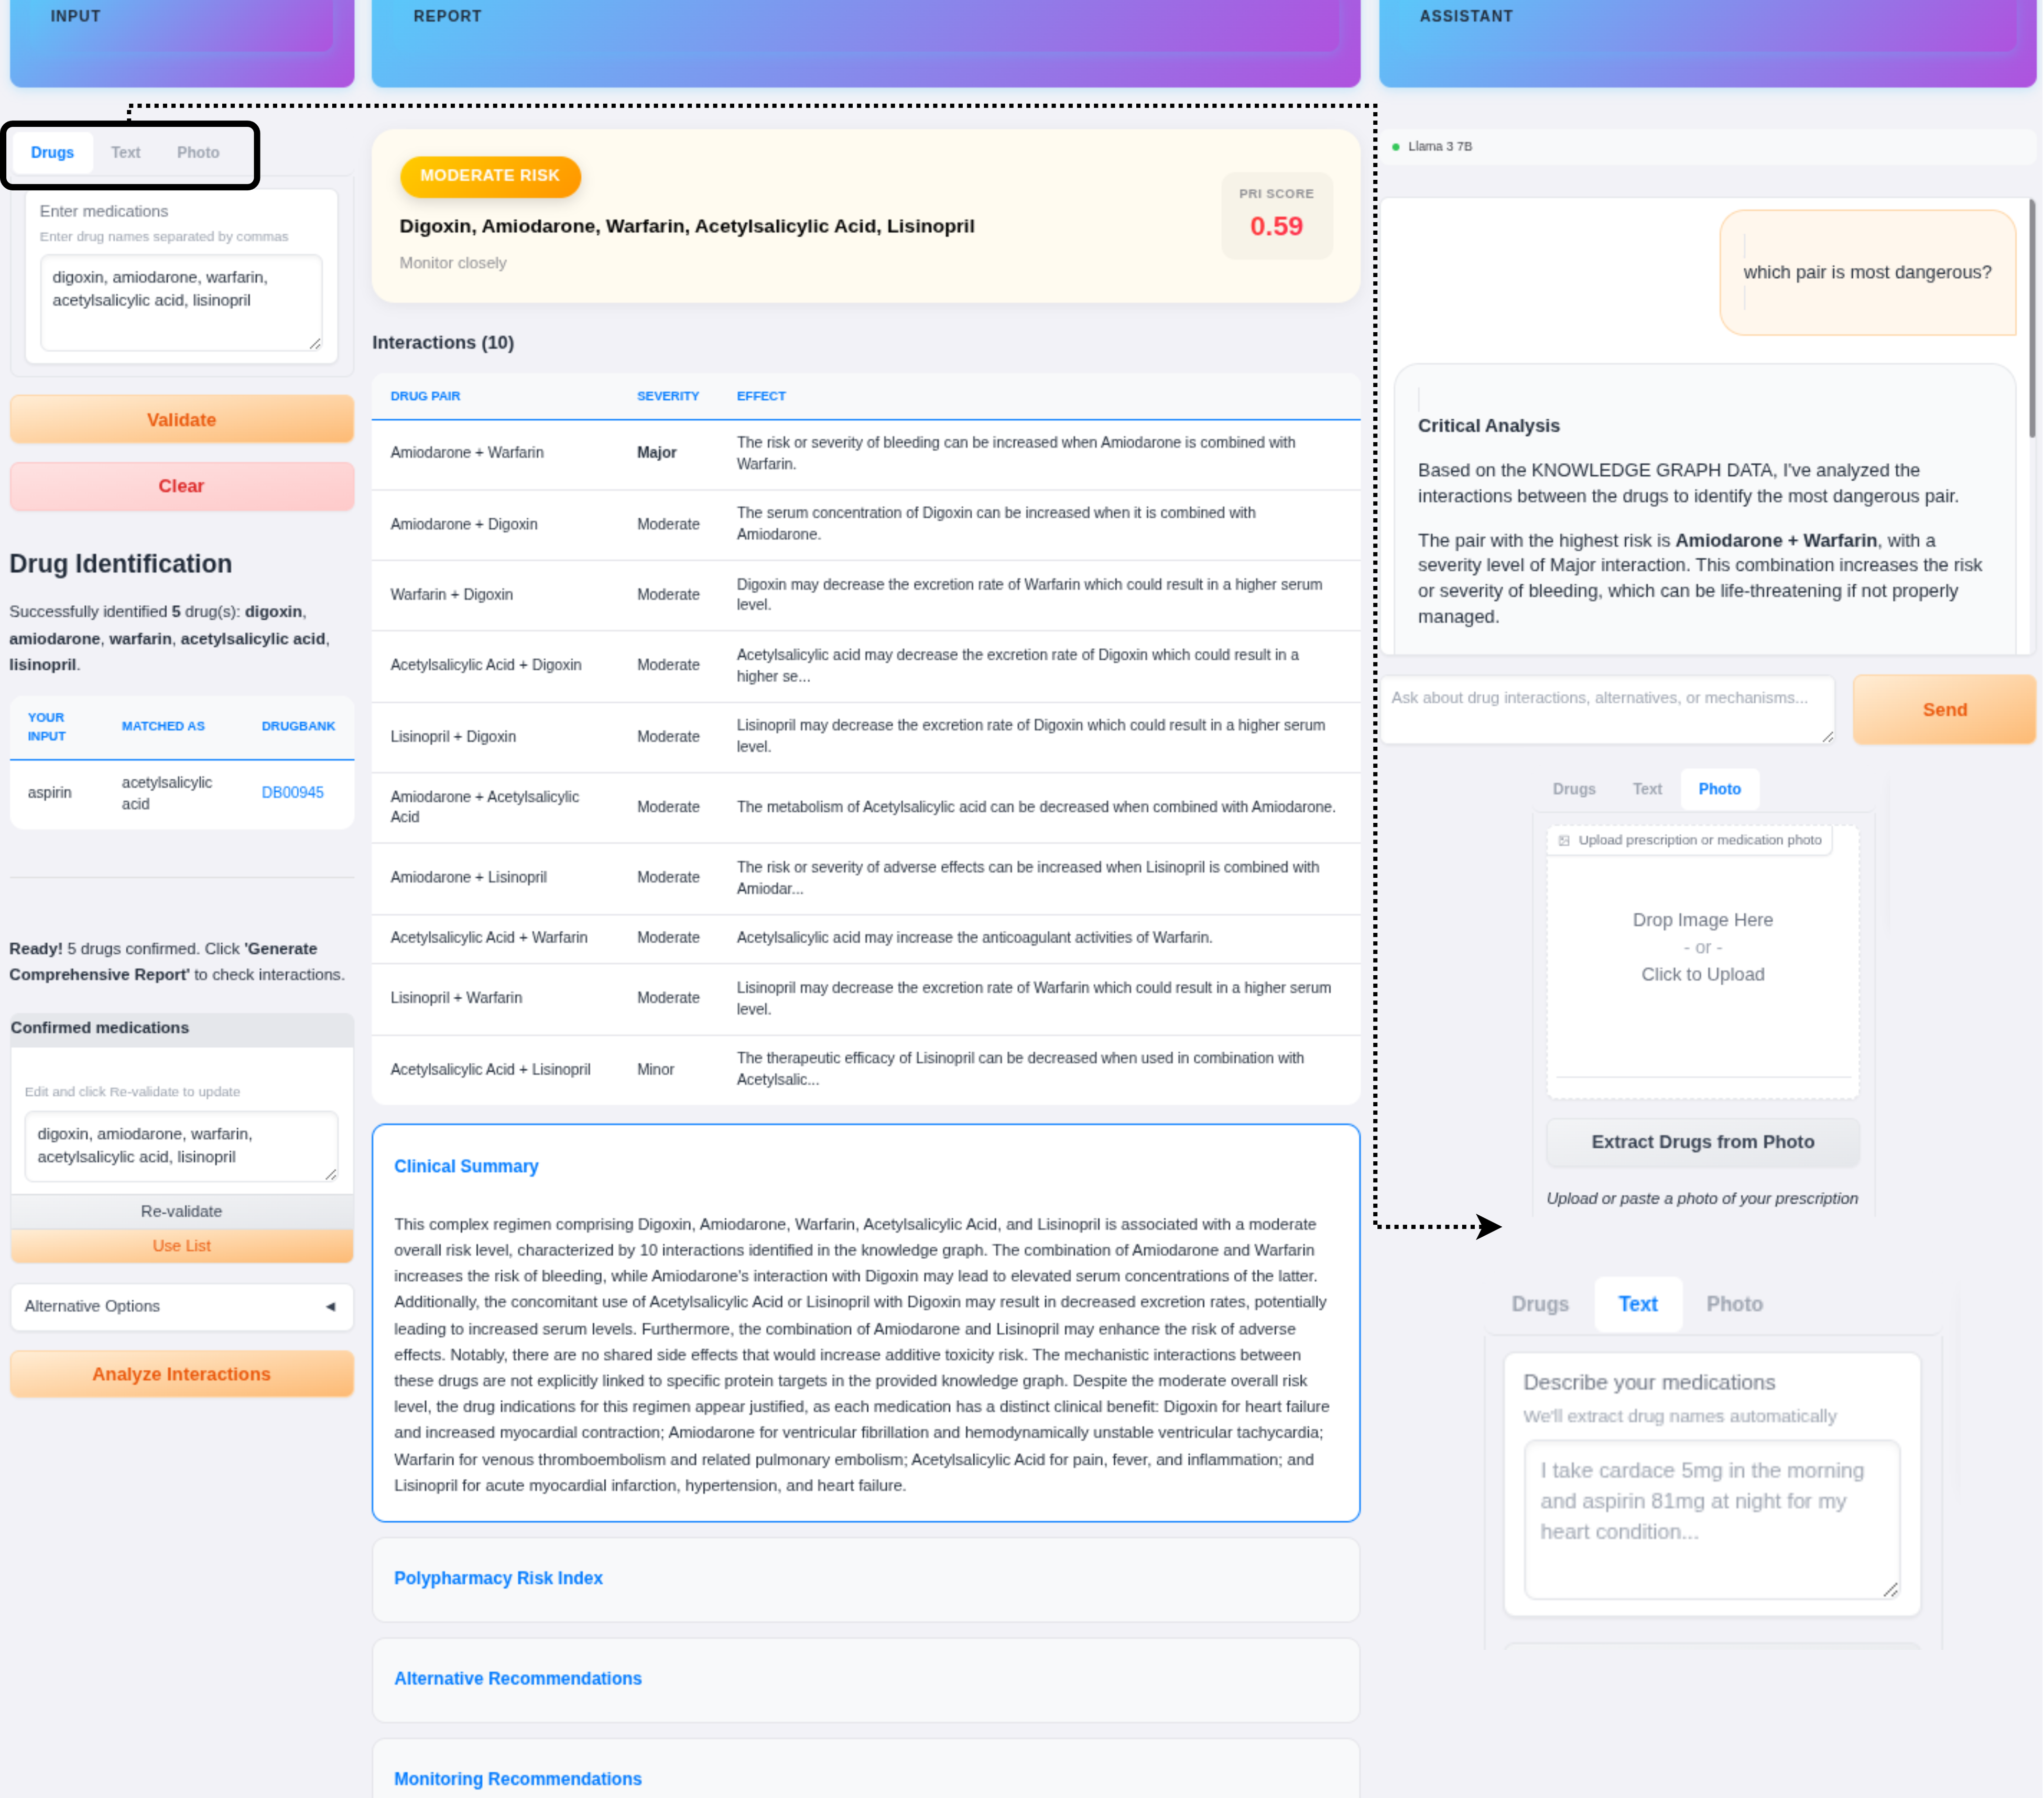
\includegraphics[width=\textwidth]{Application-diagram.png}
\caption{Screenshot of the DDI Risk Analysis Web Application demonstrating analysis of a five-drug cardiac polypharmacy regimen (Digoxin, Amiodarone, Warfarin, Aspirin, Lisinopril). \textbf{Left panel}: Drug input interface with text entry and validation. \textbf{Center panel}: Generated interaction report showing severity-classified DDI pairs under collapsible sections, with risk level assessment. \textbf{Right panel}: LLaMA 7B chat assistant responding to the query ``Which pair is most dangerous?'', with text and image input options visible at the bottom.}
\label{fig:app_demo}
\end{figure}

\end{document}
